\documentclass[a4paper, 12pt]{article}

\usepackage[utf8]{inputenc}
\usepackage{amsmath}
\newcommand{\norm}[1]{\left\lVert#1\right\rVert}

\usepackage[]{amsfonts}
\usepackage[]{graphicx}
\usepackage{wrapfig}
\graphicspath{{figures/}}

\title{CS231A Course Notes 6a: Feature Detectors}
\author{Sahaj Garg and Marcus Gomez}
\date{}

\renewcommand\emph{\textbf}

\numberwithin{equation}{section}
\begin{document}

\maketitle

\section{Introduction}
In order to perform tasks described so far in this course, such as computing homographies between images or estimating fundamental matrices, we have assumed that an oracle provided us with matching keypoints in images. In this course notes, we explore methods for constructing these matching keypoints, and more generally \textbf{detecting} and \textbf{describing} interesting features in images. By detecting and describing features, we can also match features, leading to our ability to estimate properties of the images (such as homographies or fundamental matrices), index objects, and detect instances of the same object class. Some of these applications have already been discussed, and others will be discussed in the recognition portion of this course. 

We begin by discussing useful features and how to detect them, then explain different descriptors that can be used. 

\section{Detectors}
The first step in any estimation, matching, indexing task is to detect the features we want to use for our models. Here we cover a few major types of features we might want to detect.
\subsection{Edge Detectors}
Edges capture important information about large discontinuities in properties of objects in a given observation. We filter out the majority of less relevant information while maintaining the structure of the objects in the image. Edges can identify many important changes including: 
\begin{itemize}
\item Discontinuities in depth 
\item Surface orientation discontinuities
\item Changes in surface material properties (reflectance discontinuities)
\item Illumination discontinuities (i.e. large changes in light, picking up on highlights, shadows, etc.)
\end{itemize}
Canny (1986) defines a few criteria for optimal edge detection. In particular, we want the following properties in a good edge detector:
\begin{itemize}
\item \textbf{Good detection accuracy}: we want to minimize false positive rates (detecting noise as edges) and false negative rates (missing real edges). Ideally, this means we detect as many edges in the image as possible.
\item \textbf{Good localization}: detected edges need to be detected as close as possible to the real edges. More formally, the edge point detected from the operator should accurately localize on the center of the image
\item \textbf{Single response constraint}: minimize the number of local maxima around the edge. Put another way, an edge detection operator should only mark each edge in an image once.
\end{itemize}
Keeping Canny in mind, we now actually design an edge detection operator. A simple edge detector applies some basic Gaussian smoothing to prevent gradient estimates from being too noisy, and then uses derivatives in the x and y directions to find points of high change / gradient in the image. First, let $A$ be our original image and $G$ be our Gaussian filter kernel (where $G_{xy} = \dfrac{1}{2\pi\sigma^2}e^{\dfrac{-x^2-y^2}{2\sigma^2}}$. Then, we compute the smoothed edge image as the following
$$S = \nabla (G * A) = \nabla (G) * A $$
where the $*$ operator convolves the second matrix with the first as a kernel, the second step is just a property of convolutions. Note that the second step means that we can precompute the kernel and never have to actually take a gradient in real time for edge detection.
Canny proposes a slightly more complicated four-step method as follows. Given an image $A$,
\begin{enumerate}
\item \textbf{Image smoothing}: convolve the image with a Gaussian kernel $G$ to reduce the noise. Take $A' = G * A$
\item  \textbf{Compute image gradients with Sobel}: Get first derivatives in the horizontal and vertical directions by filtering with the Sobel kernel to get $A'_x = L_x * A'$ and $A'_y = L_y * A'$, where $L_x = \begin{bmatrix}
-1 & 0 & 1 \\ -2 & 0 & 1 \\ -1 & 0 & 1\end{bmatrix}$ and $L_y = \begin{bmatrix}1 & 2  &1 \\ 0 & 0 & 0 \\ -1 & -2 & -1\end{bmatrix}$ are the regular Sobel operators. If $B$ and $C$ are the edge gradient and direction matrices respectively, then we have $$B_{ij} = \sqrt{(A'_{x})_{ij}^2 + (A'_{y})_{ij}^2}$$ and $$C_{ij} = \tan^{-1}(\dfrac{(A'_y)_{ij}}{(A'_x)_{ij}})$$
\item \textbf{Non-maximum suppression}: Even after performing the gradient calculation, we may still get a fairly blurry image, which violates the single response constraint, that says we should only detect one edge per real edge. In a good edge detector, we would detect thinner edges (corresponding to single response per edge). To correct for this, we perform non-maximum suppression. In particular, we iterate over every pixel and compare it to its neighbors in the same direction; if it isn't a local maximum in its neighborhood, its value is suppressed to $0$.
\item \textbf{Hysteresis Thresholding}: In this final stage, we apply a last layer of filtration. We maintain two thresholds -- a minimum and maximum. Edges with gradient above the maximum value are by default considered to be real edges (we call these strong edges); edges with gradient below the minimum are by default discarded. The remaining edges -- those with gradient between minimum and maximum (we call these weak edges), are kept if they are connected to some strong edge at any point. More formally, for each weak edge pixel and its 8 neighbor pixels; as long as at least one of the neighbors belongs to a strong edge, we keep the weak edge point. 
\end{enumerate}
\subsection{Corner Detection (Harris)} 
Corner detection is particularly interesting since the features are more stable across changes in viewpoint. They thus are really good features for use in tasks like matching. For any good corner or blob detector, we want the following properties:
\begin{itemize}
\item \textbf{Repeatability}: Even given geometric and photomeric transformations, we should be able to find the same feature in multiple images.
\item \textbf{Saliency}: The features should be found at interesting // important regions
\item \textbf{Locality}: Features should occupy small areas of the image (i.e. big features area-wise are no good)
\end{itemize}
\begin{figure}
\centering
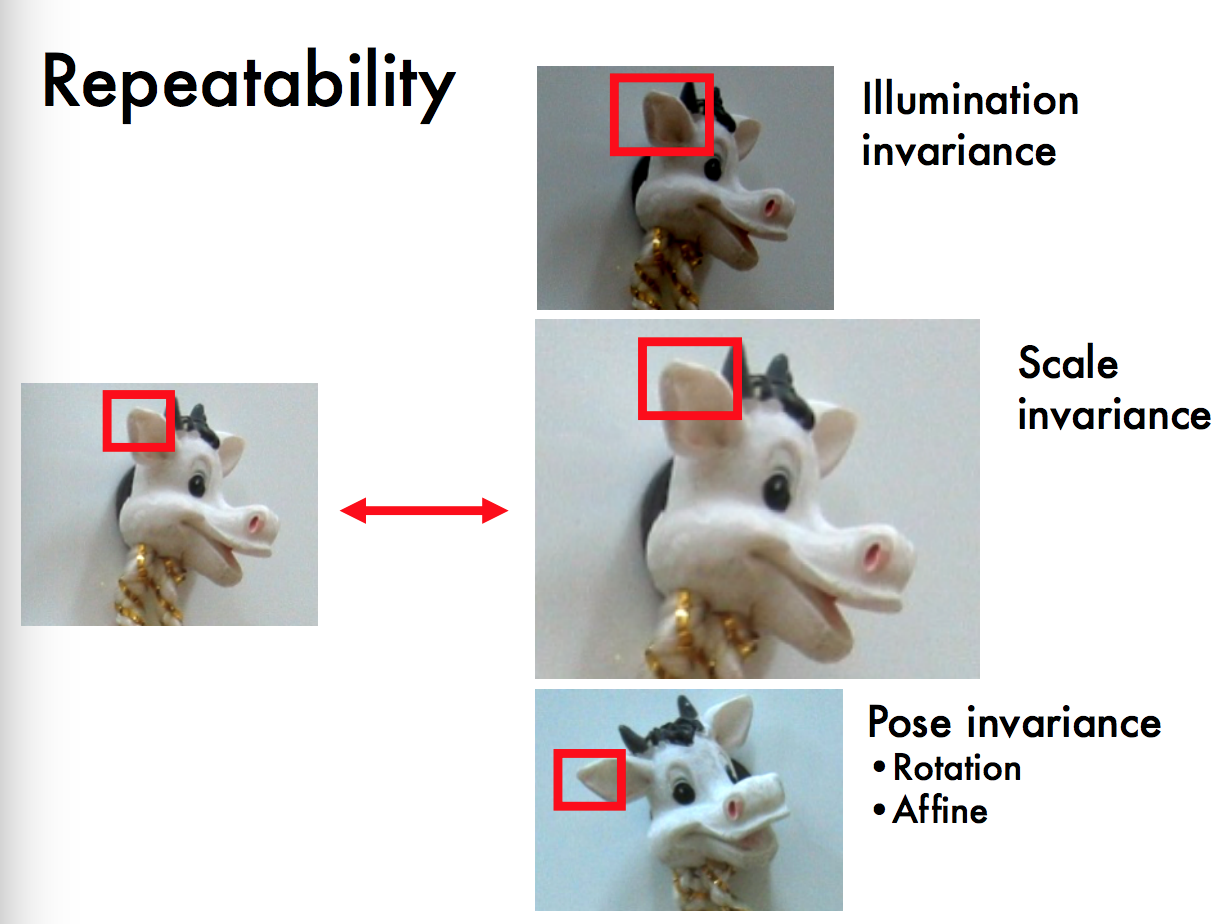
\includegraphics[width=0.5\textwidth]{repeat}
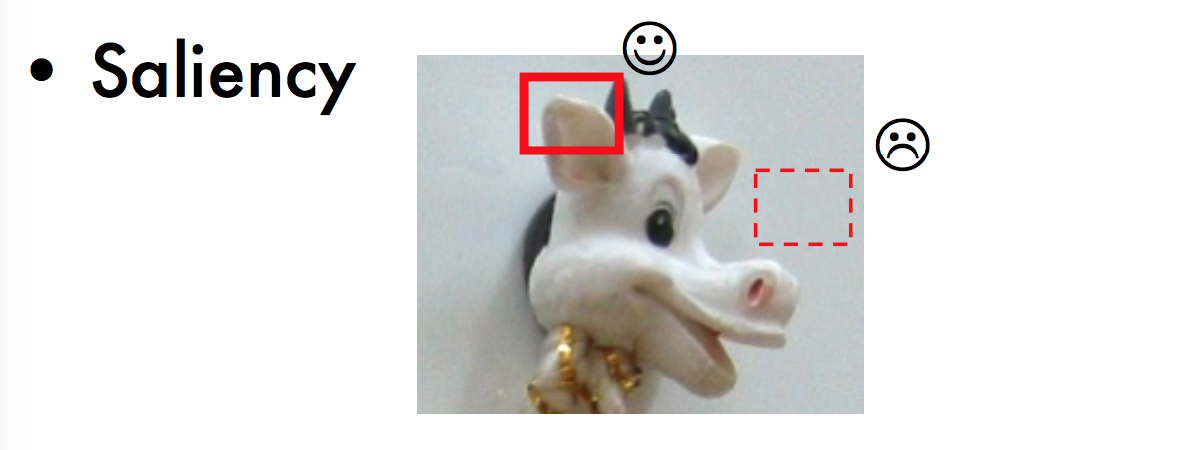
\includegraphics[width=0.5\textwidth]{salient}
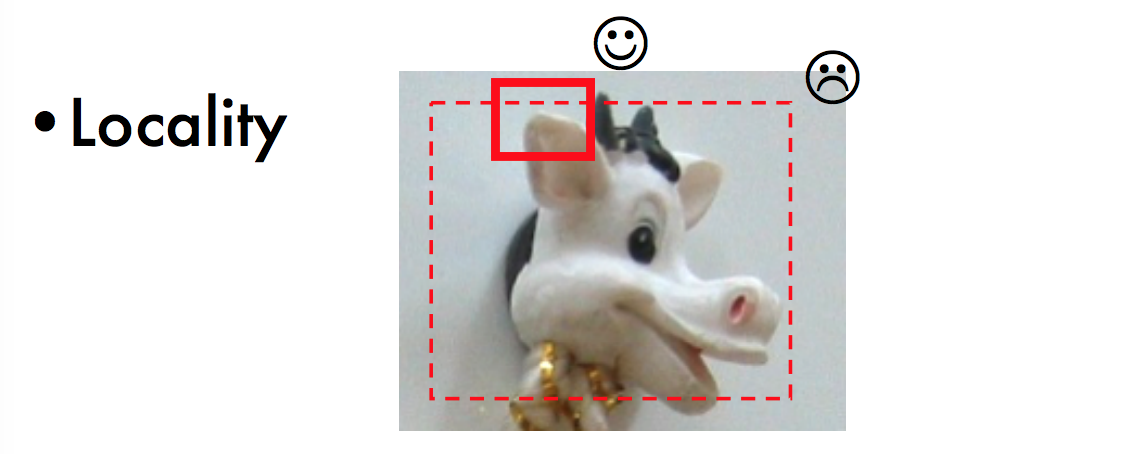
\includegraphics[width=0.5\textwidth]{local}
\caption{Good and bad examples of each of the desired feature properties for corner and blob detectors}
\end{figure}
Harris \& Stephens (1988) detail such a corner detector that has thes desired properties. In particular, they compute the intensity at $(u,v)$ as
$$E(u,v) = \sum_{x,y}w(x,y)[I(x+u, y+v) - I(x,y)]^2$$
where $w(x,y)$ is some window function that is either a rectangle or Gaussian about the center $(u,v)$. Using a Taylor expansion (left to the reader), we can then approximate $E$ as 
$$E(u,v) \approx \begin{bmatrix} u & v\end{bmatrix}M \begin{bmatrix}u \\ v\end{bmatrix}, M = \sum_{x,y}w(x,y)\begin{bmatrix}I_xI_x & I_xI_y\\I_xI_y& I_yI_y\end{bmatrix}$$
where $I_x$ and $I_y$ are the image derivatives in the x and y directions respectively. We can compute them using finite differences or, more robustly, a standard Sobel operator. At this point, we then compute the Harris response score, which is given by 
$$R = \text{det}(M) - k\text{Tr}(M)^2 = \lambda_1\lambda_2 - k(\lambda_1+\lambda_2)$$
where $\lambda_1,\lambda_2$ are the eigenvalues of $M$. We then consider three distinctions:
\begin{itemize}
\item If $|R|$ is small, we consider the region to be flat -- that is, there are no changes in any direction. This corresponds to small $\lambda_1$ and $\lambda_2$.
\item If $R < 0$, we consider the region to be an edge. This corresponds to $\lambda_1 >> \lambda_2$ or $\lambda_2 >> \lambda_1$. 
\item If $|R| >> 0$, we consider the region to be a corner. This corresponds to large $\lambda_1,\lambda_2$ and $\lambda_1 \sim \lambda_2$.
\end{itemize}
\begin{figure}
\centering
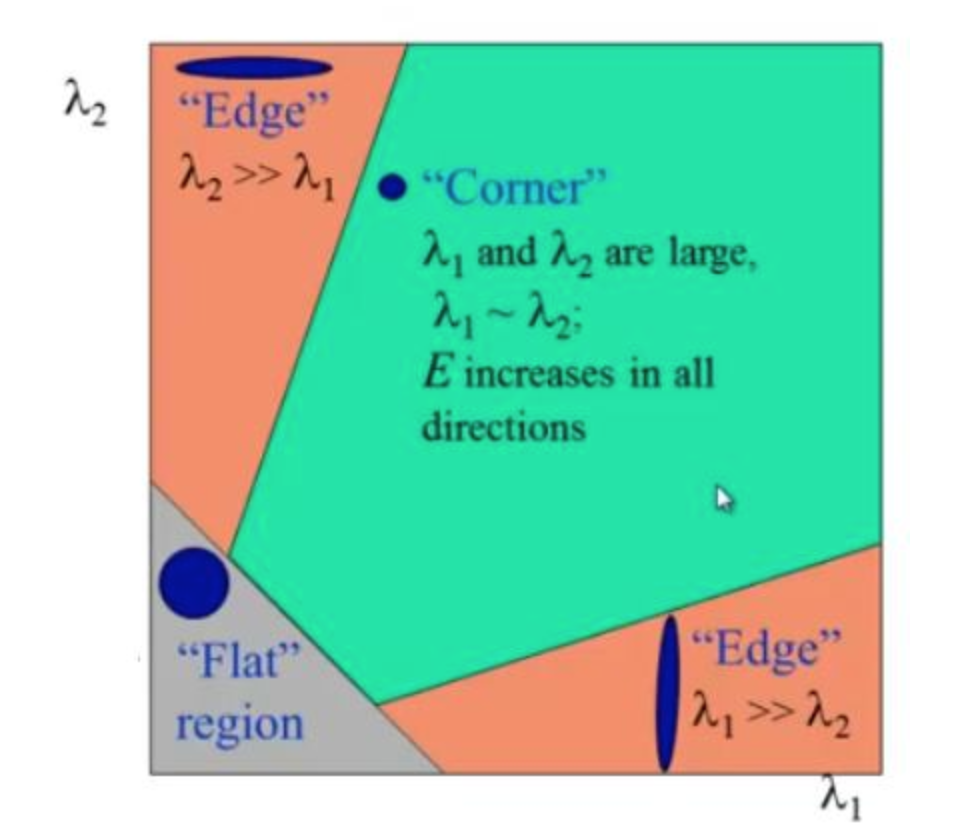
\includegraphics[scale=0.3]{h1}
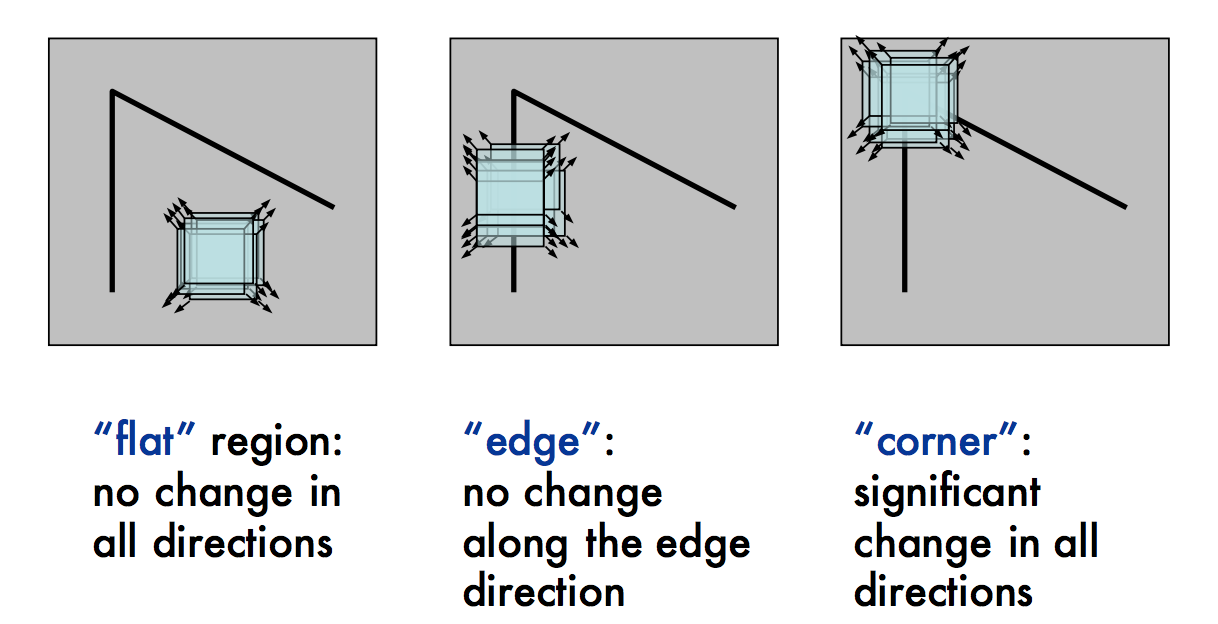
\includegraphics[scale=0.3]{h2}
\caption{Some visualizations of the three different cases for Harris corner detection scores}
\end{figure}
\subsection{Blob detection}
In a similar manner to corners, we may be interested in detecting some features that are invariant to scale -- like blobs. Like before, we consider some function $f$ that is our image, and some function $g$ be our Gaussian filter kernel. Then, instead of detection an edge as point where $f * \dfrac{dg}{dx}$ is maximum, we might detect instead an edge as $f * \dfrac{d^2}{dx^2}g = 0$. Note then that the Laplacian's magnitude is maximized at the center of a given blob in $f$ if the scale of the Laplacian is "matched" to the scale of the blob. In practice, this matching means we need to multiply the Laplacian by $\sigma^2$ (the precise reasons for this are left as an exercise to the reader); importantly, if we don't scale the Laplacian, we will likely not detect the correct maximum, as shown in the figure. As a basic example, a blob of radius $r$, the Laplacian is maximized at $\sigma = r / \sqrt{2}$. 
\begin{figure}
\centering
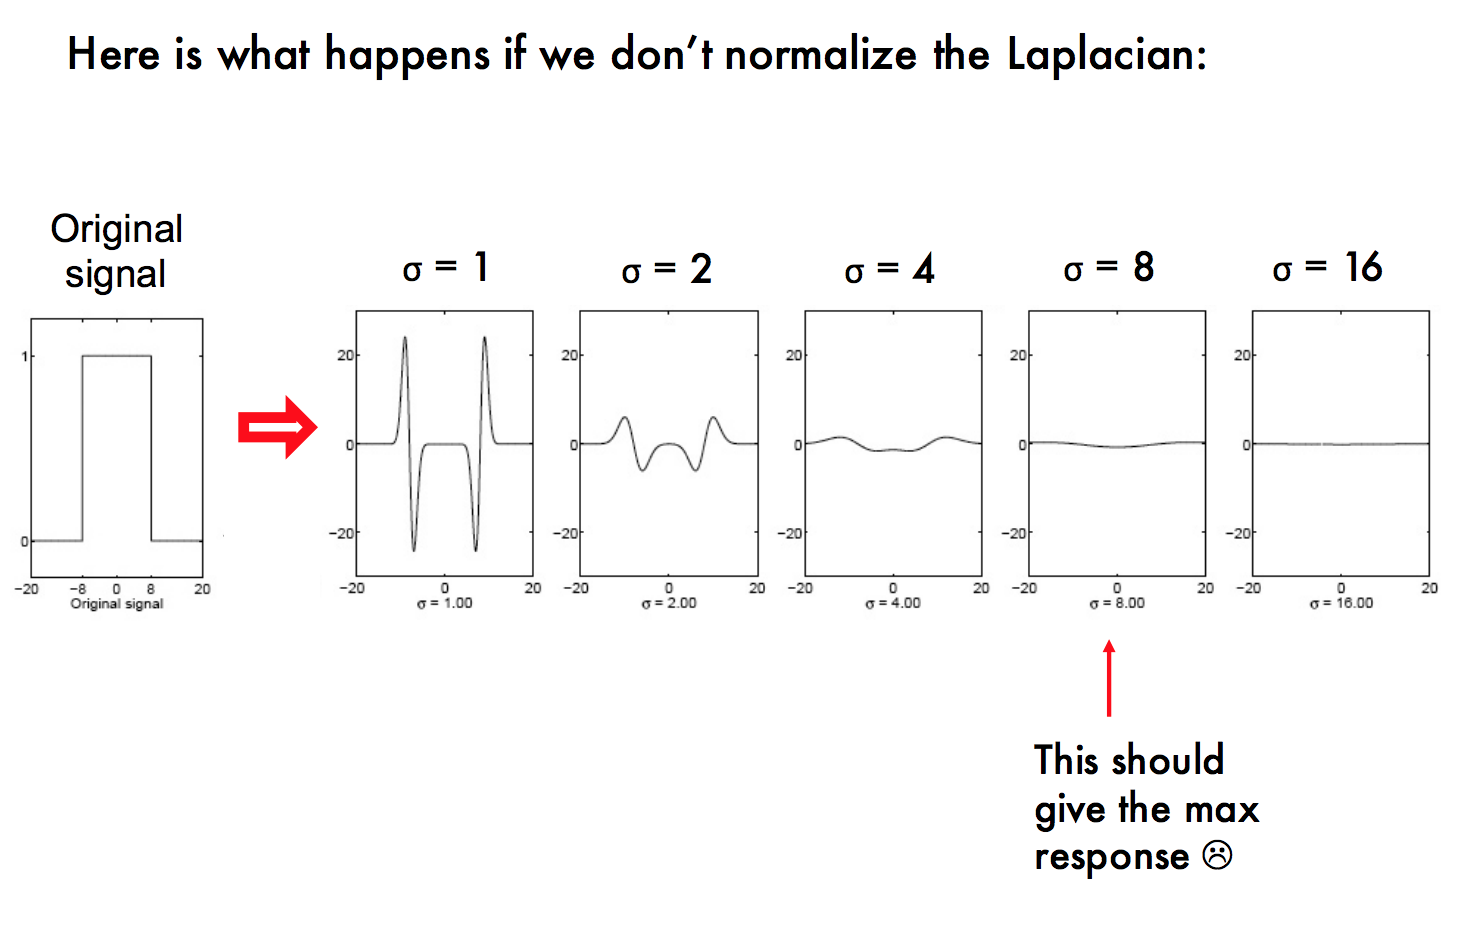
\includegraphics[scale=0.4]{scale_abnormal}
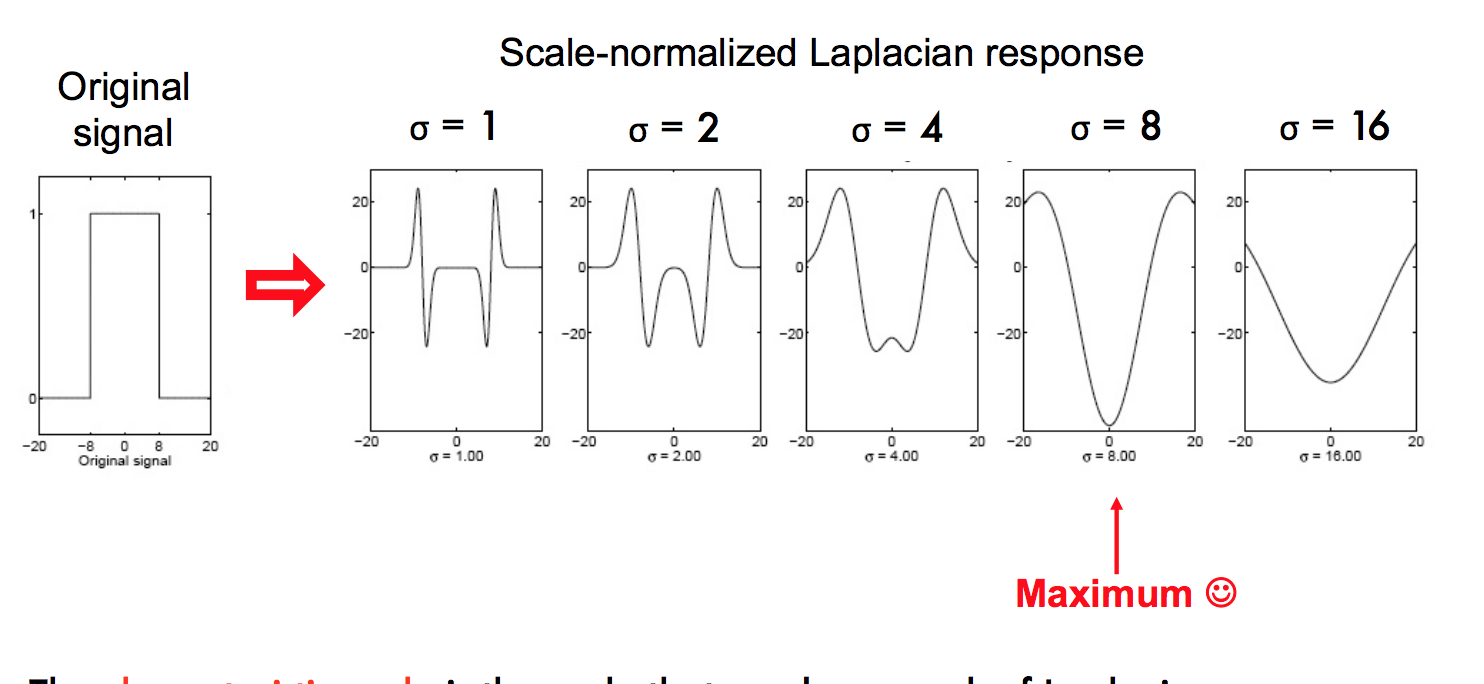
\includegraphics[scale=0.4]{scale_normal}
\caption{Forgetting to normalize the Laplacian can cause severe failure in our blob detection}
\end{figure}
As a final note, computing the Laplacian is super expensive. In practice, we typically approximate it as the difference of two Gaussians. Namely, if the Laplacian is
$$L = \sigma^2(g_{xx}(x,y,\sigma) - g_{yy}(x,y,\sigma))$$
then we can approximate
$$g(x,y,k\sigma) - g(x,y,\sigma) \approx (k-1)\sigma^2L$$


\end{document}